\documentclass[11pt,titlepage]{article}
\usepackage[pdftex]{graphicx}

\newcommand{\Pic}[2][0.85]{\begin{center}\includegraphics[width=0.8\textwidth,height=#1\textheight,keepaspectratio]{#2}
  \end{center} } 
\newcommand{\Lpic}[2][0]{\begin{center}\includegraphics[width=0.8\textwidth,angle=#1,keepaspectratio]{#2}
  \end{center} } 


\title{{\bf TITAN2D User Guide}\\ Release 1.030814}
\author{Geophysical Mass Flow Group (GMFG), University at Buffalo, NY, USA}

\begin{document}

\maketitle

\tableofcontents

\newpage

\section{Introduction to TITAN2D}

TITAN2D is a program developed for the purpose of simulating dry
granular avalanches over digital interpretations of natural terrain.
The program is designed for simulating geological flows such as debris
avalanches and landslides.  TITAN2D combines numerical simulations
with simulated natural terrain supported through a Geographical
Information System (GIS) interface.  TITAN2D represents the latest
research in numerical modeling and parallel computing with integrated
support through a GIS [Patra et al. 2003]

The TITAN2D program is based upon a model for an incompressible
Coulomb continuum, a ``shallow-water'' granular flow [Iverson and
Denlinger, 2001].� The conservation equations for mass and momentum
are solved with a Coulomb-type friction term for the interactions between
the granular material and the basal surface [Savage and Hutter,
1989].� It is assumed that conservation of energy can be neglected to
the first order because the coarse grain size typical of the basal
avalanche results in minimal thermal effects on avalanche propagation.
The resulting hyperbolic system of equations is solved using a
parallel, adaptive mesh [Berger and Colella, 1989], Godunov scheme [Davis, 1988].� The Message
Passing Interface (MPI) [http://www-unix.mcs.anl.gov/mpi/] Application
Programmers Interface (API) allows for computing on multiple
processors, increasing computational power, decreasing computing time,
and allowing for the use of large data sets. Adaptive gridding allows
for the concentration of computing power on regions of special
interest. Mesh refinement captures the leading edge of the flow, as
well as locations where the topography changes rapidly.  Mesh
unrefinement is applied where solution values are relatively constant
or small to further improve computational efficiency.

The model used in TITAN2D assumes a continuum volume, parcels of which are pulled downslope by
gravity.  Friction between particles and between particles and ground resist this
momentum. Governing equations for this model, the conservation of
mass and conservation of momentum, are solved using approximate numerical solution methods, e.g. finite volumes etc. The outputs of TITAN2D are flow
momentum (h/v), depth, run-up height, and inundation area.

TITAN2D operates via a python scripted Graphical User Interface (GUI).
Through this interface the user inputs the parameters needed to
sucessfully run the program such as pile dimensions, starting
coordinates, internal and bed friction angles, and simulation time.
The simulation is computed on a Digital Elevation Model (DEM) of the
desired region and results can be displayed through the TITAN2D viewer
utility, or other visualization software packages.

\section{Getting Started}

\subsection{TITAN2D program file}

The latest edition of the TITAN2D program can be obtained from fire.ccr.buffalo.edu.  Upon entering your home directory on ``Fire'', type
the following command line (using year-month-date format): ``cvs
export -D yyyy-mm-dd gmfg''.  To get the most recent
version of the program add a day to the current date.  For example if
today's date is April 1, 2003, type: ``cvs export -D 2003-04-02
gmfg''.  After the ``gmfg'' directory
has been created and added to your home directory, it can be
transferred to the computer of your choosing.  Major releases of TITAN2D can also be obtained from the GMFG website [gmfg.buffalo.edu].

\subsection{GRASS GIS Data file}

TITAN2D performs flow simulations on a DEM of a user-defined region.
The DEM file containing X,Y,Z data (typically latitude, longitude and
elevation in meters) must be properly configured to operate with
TITAN2D through the use of a header.  The DEM data file is then
formatted to operate in a GRASS (Geographic Resources Analysis Support System) GIS environment.  GRASS GIS is an open source GIS with raster, topological vector, image processing, and
graphics production functionality.  It operates on various platforms
through a graphical user interface and shell in X-Windows.  GRASS is available free of charge under GNU General Public License (GPL)
[http://grass.ibiblio.org/index.html].

Simulation accuracy is highly dependent on the level of DEM resolution
and quality.  DEMs with higher resolutions (e.g. 5-30m) render more
accurate representations of actual geophysical flow events, especially
in situations where channelized flow is involved.

The GRASS GIS interface used in conjunction with TITAN2D allows the
user to adjust the area of the desired initial DEM.  This capability
decreases output file size thus increasing visualization speed and
allows the user to focus attention upon a specific region of interest
within a much larger DEM.

\section{Instructions for Using TITAN2D}

After obtaining the latest version of TITAN2D and configuring a GRASS DEM of the desired
region, the user is ready to simulate a geologic flow event.  First,
go to the ``./titan/bin/'' directory.  Then type ``{\bf python titan\_gui.py}''.  This command will open the TITAN2D GUI.
  

\subsection{TITAN2D Graphical User Interface (GUI)}
Figure 1 shows the GUI for TITAN2D.  The user inputs information into the boxes prior to running the simulation. The information required falls into one of three types: 1) GIS data specifications, 2)
Computational parameters and 3) Pile parameters (of the initial flow
mass).

\begin{figure}[h!]
  \Pic{gui_1}
                \caption{ Sample Python2 Graphical User Interface (GUI)}
                \label{ht1}
                \end{figure}


\begin{enumerate}
\item{} Specifying the GIS Information: The first four options ask the
  user to input information on the GIS data to be used in the
  simulation:
  
  The \underline{{\bf GIS Information Main Directory}} box displays
  the location of the GIS datasets. For example, this may be
  ``/computer\_naimage\_epsme /home/username/directory\_name/grass.data/grass5/''.  The directory ``./grass5/''
  is the top GIS directory in which all the data is stored.  Within
  this directory, subdirectories containing separate datasets are
  found. When running the simulation, a specific subdirectory is
  entered into the \underline{{\bf GIS Sub-Directory}} box.
  
\item{} The \underline{{\bf GIS Map Set}} and \underline{{\bf GIS
      Map}} point to the DEM dataset that the user chooses to use in
  the simulation. As shown in Figure 2, they are in the same
  sub-directory, ``./ColimaSRTM/''.

\begin{figure}[h!]
  \Pic{gui_2}
                \caption{ Entering GIS data into Graphical User Interface}
                \label{ht1}
                \end{figure}
                
              \item{} The Computational Parameters: The next inputs
                relate to the actual computation and output of the
                data. The \underline{{\bf Simulation Directory
                    Location}} specifies the directory where the
                output data files will stored (see Figure 3).  A
                directory must be specified in this box. If the
                specified directory already exists, it will not be
                overwritten and data will not be submitted for
                processing.  The specified directories are found relative to                                    the ``/computer\_name/home/username/directory\_name/
                titan/bin/'' directory. For example, the
                directory path would be ``./bin /colima\_example/''
                and the specified directory would be
                ``./colima\_example/''. Every time the simulation
                runs, a new simulation directory must be created.

\begin{figure}[h!]
  \Pic{gui_3}
                \caption{ Entering Computational Data into the Graphical User Interface }
                \label{ht1}
                \end{figure}

                
                The number of processors that the user decides to use
                must be specified in the \underline{{\bf Number of
                    Processors}} box. If more than one processor is
                specified, each gets a share of the processing load,
                thus decreasing simulation run time. However, if too
                many processors are specified, the data submitted may
                be queued until the number of chosen processors become
                available.  The user must be aware of the number of
                available processors on any given machine.
                Crosby.ccr.buffalo.edu for example, offers a maximum
                of 8 processors.  An excellent website to check the
                status of Center for Computational Research (CCR)
                machines is:
                http://www.ccr.buffalo.edu/Hotpages/hotpage\_main.html.
                At this site one can find out how many processors a
                particular machine offers as well as its current
                workload.
                
                TITAN2D creates a regular grid/mesh on which the
                computation is done with the size specified by the
                user in the {\bf Computational Mesh Points in
                  Y-Direction} box. The user specifies the number of
                points in the Y-directions and the code calculates the
                number of grid points needed in the x-direction in
                order to have a regular grid.  When large numbers of
                grid points are specified (e.g. in excess of 500), the
                more computational time is need to process the data
                and the more disk space is needed to store the output
                files.  A compromise must be found in terms of
                computation time and computation grid resolution
                (based on the size of the DEM dataset).
                
                The next two parameters needed are the two angle
                values used in the computation of a simulation. The
                {\bf Internal Friction Angle} and the {\bf Bed
                  Friction Angle}, specified in degrees, control the
                resistance to flow of the event being simulated.  If
                the flow being simulated originates from more than one
                source, or if the user wishes to simulate more than
                one flow simultaneously in different locations, the
                {\bf Number of Piles} must be specified. If only one
                flow is being simulated or a single source area is
                needed, then insert a value of 1. The dimensions and
                locations of the pile(s) are specified when this first
                stage is completed.
                
                TITAN2D allows for several properties of the
                simulation to be scaled.  Clicking the {\bf Scale
                  Simulation} button (button turns red when selected),
                allows the governing equations to be scaled by the
                pile height, gravity and a length scale. The pile
                height scale is taken from the Pile Height input so
                that the initial pile height is assumed to be the
                maximum and scaled to 1. Gravity is also scaled to 1.
                If this button is not selected, Gravity is 9.80 m
                s$^{-2}$ and the pile heights are then calculated.
                Unlike the pile height and gravity scales that are
                computed automatically by the code, the user must
                specify the length scaled in the \underline{{\bf If
                    Scaled, Length Scale (m)}} box. This scaling
                refers to the run out length of the flows. This need
                only be specified if the simulation is to be scaled, however for all real-terrain calculations it is highly recommended that the simulation be scaled.

                
                The next two input parameters concern the run time of
                the simulation. The user must specify the
                \underline{{\bf Maximum Number of Time Steps}} (on the
                order of several thousand) and \underline{{\bf Maximum
                    Time}} (in seconds). When the job is submitted for
                processing, the simulation will stop when it has gone
                through the time steps or has been running for the
                specified amount of time. The program has the
                potential to output a data file for every time step it
                goes through. This is usually unnecessary as the files
                can take up vast amounts of disk space and there may
                be very little change from one time step to the next.
		
		{\bf * A Note on setting the maximum time and maximum number of time steps:}
Determining an acceptable stopping criteria for the simulation is
difficult when considering general cases.  Because of this, the stopping
criteria for the simulation must be set by the user.  The two criteria
that are used are {\bf Maximum Time} and {\bf Maximum Number of Time Steps}.  Both of
these values should be set high enough such that the geologic event being
simulated has ended (e.g. the material has come to rest).  If either of
these values are set too low, the simulation will end with the material
not having reached static equilibrium.  If both of these values are set
excessively high, wasted computation will be performed dynamically
simulating the pile in static equilibrium.  The simulation will end when
either the number of time steps computed is equal to the Maximum Number of
Time Steps or the simulation time has reached the Maximum Time.  The
number of computed time steps needed to simulate a geologic event will
vary depending on the amount of computational mesh points used, the
friction parameters, the use of grid adaptation, the simulation order, and
initial pile geometry and location.

                In the \underline{{\bf Time Steps per Results Output}}
                box, the user can specify how often an output file is
                to be created. For example, the user may wish to
                generate an output file every 100 time steps.  The next 
                box in this section is the \underline{{\bf Adapt the Grid?}}                                    option. This refers to the
                computational grid and improves the simulation
                accuracy while decreasing the computational cost.
                However, this can also introduce some instability into
                the computation.  Due to the major savings in computation, it is recommended that this be selected unless instability is detected in the output.
                
                The \underline{{\bf Visualization Output}} box allows
                the user to choose the formats of the output files
                (tecplotxxxx.plt/mshplotxxxx.plt/ GMFG Viz/HDF/Web
                Viz) - Activate the buttons corresponding to the
                visualization outputs that are desired.
                Tecplotxxxx.plt and mshplotxxxx.plt are tecplot files [www.amtec.com].
                GMFG Viz is for the TITAN2D visualizer.  HDF is for
                HDF5 output.  Web Viz is for the web visualization
                output.  The user can have multiple visualization
                output formats with each simulation run.
                
              \item{} 1st/2nd Order Options: Clicking on the
                \underline{{\bf Second}} button for this option allows
                you to select the 2nd order method for calculating the
                values in a computational grid cell (the 1st order
                method is the default). Under the first order method,
                the values for pile height, momentum etc. that are
                calculated by the model are approximated as constant
                across the entire cell. This may mean that there is a
                jump up or down to the value of the same parameter in
                the neighboring cell. Under the 2nd order method, the
                values of the parameters are assumed to vary linearly
                across the cell. The 2nd order method takes into
                account the value of the neighboring cells and uses
                those values to calculate the value for the cell in
                question. For example, if the neighboring cells
                up-flow of the cell in question have values lower than
                the cells down-flow of the cell in question, the value
                of the cell is going to increase (have a slope) in the
                down-flow direction. If there is no difference in
                values between the neighboring cells, then the cell in
                question will also stay constant. Selecting the 2nd
                order method will produce slightly more accurate
                results, but may also increase the computation time as
                the code has to perform more calculations.
                
                The \underline{{\bf Minimum (and Maximum) x and y
                    location (UTM E, UTM N)}} boxes can be used if a
                computational region smaller than the entire GIS
                region is desired, the user can input the minimum and
                maximum x and y location of the desired computational
                region in UTM coordinates.
                
                When the simulation has finished running, the user
                will be notified via the email address specified in
                the \underline{{\bf Email Address}} box. If an address
                is not set, notification will be sent to
                user@buffalo.edu. An email notification in not sent if
                TITAN2D is being used on a PC.
                
                The \underline{{\bf Clean}} button will remove any
                excess object files, executables and data files.
                Cleaning should be done periodically to purge excess
                files to prevent errors from being introduced into the
                computation. The \underline{{\bf Run}} button begins
                the submission of the data to the processors. When
                this button is selected, a new window appears (figure
                4), in which the user specifies the various parameters
                for the pile dimensions and locations (see section
                below). The \underline{{\bf Quit}} button exits from
                the GUI and code, while the \underline{{\bf ?}} button
                opens a new window displaying help files for this
                particular GUI.


\begin{figure}[h!]
  \Pic{gui_4}
                \caption{ Entering Pile information into Graphical User Interface}
                \label{ht1}
                \end{figure}
                
              \item{} Pile Dimensions: Figure 4 shows the secondary
                window used for specifying the pile dimensions and
                locations. As described earlier, this window is
                generated when the \underline{{\bf Run}} button is
                selected in the main window.  The first line in the
                window states the pile number for which the dimensions
                are being entered. In order for the user to specify an
                initial pile geometry that can vary, the pile is
                assumed to have the shape of a paraboloid given by the
                equation $P*(1-((x-xc)/xr)^2 - ((y-yc)/yr)^2)$.  The
                data to be entered by the user are: \underline{{\bf
                    Pile Thickness}} (in meters), \underline{{\bf
                    Location of the Center of the Pile}} (in UTM
                coordinates) and the \underline{{\bf Pile Radius}} in
                the X and Y directions (in meters).  If two or more
                piles are being used and they overlap, the larger of
                the two pile heights will be taken as the pile height
                at the grid point.  There are three buttons on the
                bottom of this window. When the \underline{{\bf Done}}
                button is selected, the pile parameters are entered
                into the code. The \underline{{\bf Quit}} button will
                close the pile dimensions window and all the data is
                submitted to the processors for computation. If more
                than one pile needs to be specified, a new pile
                dimension window will appear when the \underline{{\bf
                    Quit}} button is selected. Once the parameters for
                all the piles have been specified, then the data will
                be submitted.  The \underline{{\bf Calculate Volume}}
                button (figure 5) will calculate the volume for the
                individual piles using the pile height and the X and Y
                extents. The volume is given in cubic meters and
                assumes there are no overlapping piles.
\end{enumerate}


\begin{figure}[h!]
\centerline{  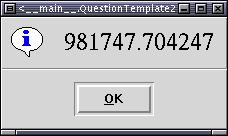
\includegraphics[scale=0.5]{gui_5}}
                \caption{ Calculated Volume Pop-Up Window }
                \label{ht1}
                \end{figure}

                
\subsection{Using TITAN2D through the GRASS GIS Interface}

TITAN2D has the unique capability of running within a GRASS GIS
environment.  Within a GRASS environment the user is able to
graphically access available DEMs, choose a specific region of
interest within a DEM, and choose a starting point for the initial
pile.  GRASS can be operated by either interactive or command-line
operations.  This function is available to the user as long as a copy
of Grass5 is installed on your computer.

\begin{enumerate}
\item{} Start GRASS GIS at the prompt with the command: ``{\bf
    grass5}''
  
\item{} Specify the location of the GRASS mapset by clicking on the
  desired DEM file name in the pop-up window (figure 6).

\item{} Change your working directory to titan/bin
  
\item{} Ensure the following files are present in the
  titan/bin directory:

\begin{enumerate}
\item{} pilehelper
\item{} regionhelpery
\item{} r.gmfg.titan2D
\item{} runit.py
\end{enumerate}
\end{enumerate}

\begin{figure}[h!]
  \Pic{grass_01}
                \caption{ GRASS GIS mapset selector window }
                \label{ht1}
                \end{figure}
                
\subsection{Command-Line Operation}

\begin{enumerate}
\item{} Specify simulation parameters on the command line for
  ./r.gmfg.titan2D, to get a list of available options and parameters,
  type: \texttt{run r.gmfg.titan2D -h}
  
\item{} After python GUI pops up (figure 7) input simulation
  parameters as usual.

\begin{figure}[h!]
  \Pic{grass_2}
                \caption{ Python Interface with GRASS functions activated }
                \label{ht1}
                \end{figure}

              \item{} Example of the model command line:
                
              \item \texttt{./r.gmfg.titan2D -a -s map=Tahoma30
                  dir=tempe mp=1 mesh=100 iang=30 bang=15 length=8000
                  maxts=1000 maxtime=100 outts=100
                  outfmt=tecplot,mshplot,HDF piles=1 pileh=50}
                
              \item {\bf Specifying the region for the simulation:}
                
              \item  Start GRASS monitor either from GRASS GUI or
                using GRASS command: \texttt{d.mon start=x0}
                
              \item  Display any map on the monitor with the
                command: ``d.rast map\_name''
                
              \item  Specify the region interactively using
                command:
                ``d.zoom''\\
                
              \item {\bf Interactive Operation of The Model}
                
              1.  Start the model from within GRASS using the
                following command: ``{\bf ./r.gmfg.titan2D}''
                
              Optionally, you can specify any command line
                options for the model and they will be reflected in
                the GUI.

                
                2.  Specify a mapset either by typing its name into
                the text field on the GUI or by clicking on the button
                \underline{{\bf Mapsets}} and selecting from the drop
                down menu.
                
                3.  Specify a DEM either by typing its name into the
                text field on the GUI or by clicking on the button
                \underline{{\bf Maps}} and selecting from the drop
                down menu.

\begin{figure}[h!]
  \Pic{grass_4.png}
                \caption{ Original DEM }
                \label{ht1}
                \end{figure}


                
                4.  Press the \underline{{\bf Region}} button on the
                on the GUI.  You can untoggle the \underline{{\bf New
                    Monitor}} button if you want to reuse your active
                GRASS monitor.
                Specify the region of interest from the original DEM (figure 8).  Figure 9 exhibits ``zooming in''on a region of interest by using the following sequence of mouse clicks to draw a box around the region:\\
                
                
                

                \indent 1) {\bf left button:} 1st region corner\\
                \indent 2) {\bf middle button:} 2nd region corner\\
                \indent 3) {\bf right button:} accept the region\\

\begin{figure}[h!]
\centerline{  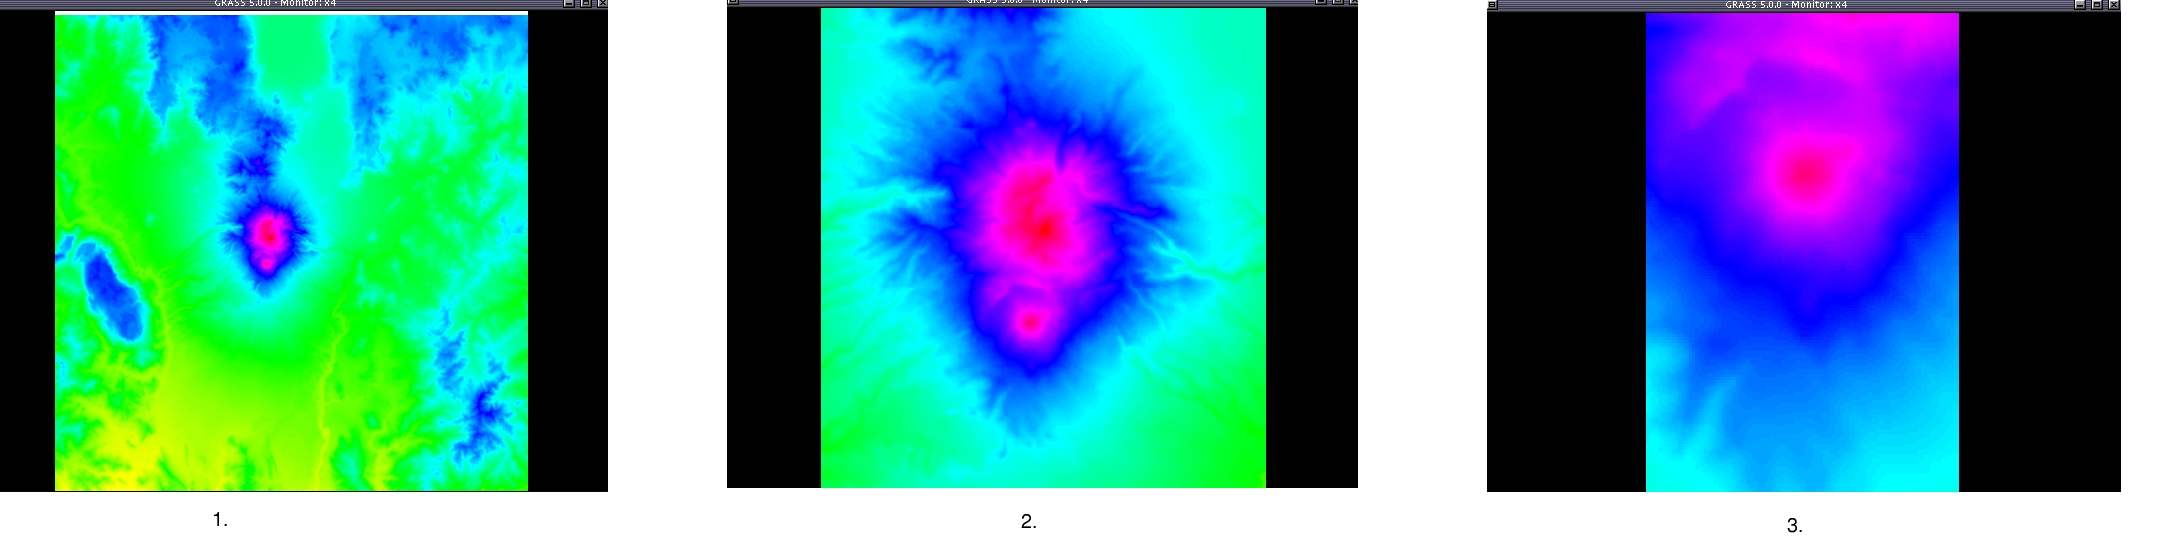
\includegraphics[scale=0.2]{grass_6}}
                \caption{Zooming in on a desired region within a DEM }
                \label{ht1}
                \end{figure}
                
              5.  Fill in the model parameters and press the
                \underline{{\bf Run}} button.  After that you will be
                presented with a pile dialog.
                
              6.  To specify pile location interactively, press
                the \underline{{\bf Map}} button on the dialog.  You
                can untoggle the \underline{{\bf New Monitor}} button
                if you want to reuse your active GRASS monitor.  After
                a map screen appears, click on the best estimated pile
                location using the left mouse button.  The coordinate
                of the point clicked will appear in the dialog box.

\end{enumerate}


\section{TITAN2D Viewer}

\begin{enumerate}
\item The TITAN2D viewer uses Open Inventor graphics libraries.  These
  libraries come preinstalled on SGI machines. However, they will need
  to be installed onto Linux machines.
  
\item To check if your machine has Open Inventor installed on it, at
  the terminal type ``{\bf ivview}'', if you see a viewer pop up,
  inventor is installed. If the command is not recongnized, Open
  Inventor needs to be installed. You can download the rpm
  distribution of Open Inventor at http://oss.sgi.com/projects/
  inventor/.
  
\item After you have ensured that Open Inventor has been installed on
  the machine, you will need to build the viewer from source on your
  platform. To do this, navigate to the directory containing the
  viewer and its source files and type ``{\bf make}''. You should see
  an executable named ``{\bf Viewer}'' in that directory.
  
\item \underline{{\bf To start using the viewer}}: place the
  simulation files in the same directory as the executable. The data
  files required by the viewer are the tri\_output*.out files
  generated by the simulation.  These files will be named ``{\bf
    tri\_outputXXX.out}'' where, the last three digits denote the
  processor number. Check to see how many of these files have been
  created by the simulation. Also place the GIS image of the terrain
  (.rgb format) in the same directory.
  
\item Now at the terminal type ``{\bf ./Viewer}''. You will be asked
  for the ``{\bf Number of Processors}'' used for the simulation
  (number of tri\_output files). Enter the appropriate number at the
  prompt. A viewer such as that shown in figure 10 will appear.


\begin{figure}[h!]
\centerline{  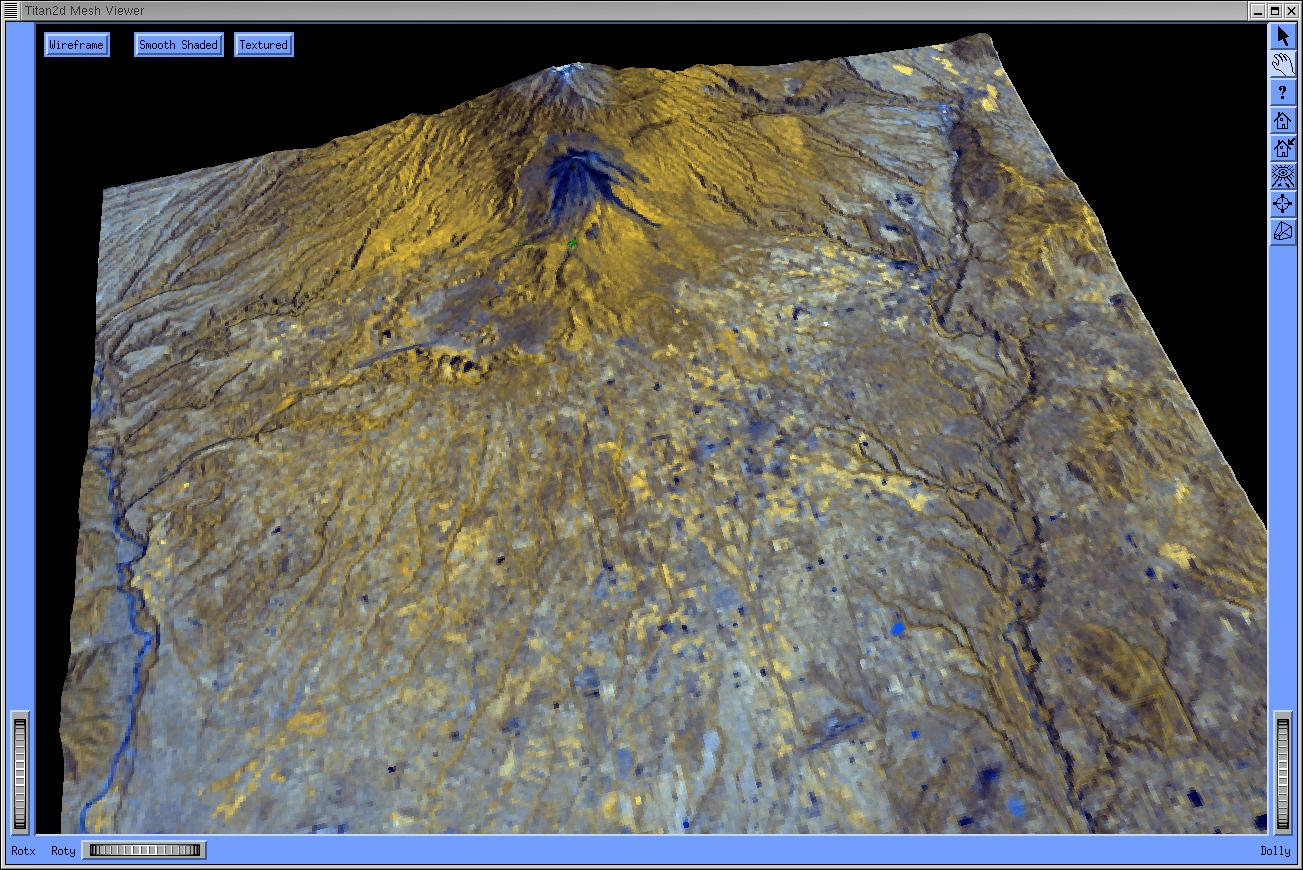
\includegraphics[scale=0.3]{screen_shot_textured}}
                \caption{TITAN2D Viewer}
                \label{ht1}
                \end{figure}

                
              \item The three buttons on the top left corner of the
                viewer allow the user to toggle between {\bf
                  wireframe}, {\bf solid} or {\bf textured} displays
                of the terrain.
                
              \item The three dials on the bottom edges of the viewer
                are provided for easy navigation (rotation, zooming)
                through the data.
                
              \item {\bf The buttons on the right edge of the viewer
                  are (from top to bottom):}

\begin{enumerate}
  
\item To allow the user to pick geometry (disabled)
\item Track ball to rotate and move through the geometry.
\item Help.
\item Reset to home viewing position.
\item Setting the home viewing position.
\item View all - View all the geometry in the data.
\item Crosshair - To zoom into a selected region in the terrain.
  Click this button and click under the area in the window that needs
  to be magnified.
\item Toggle between orthographic and perspective viewing.
\end{enumerate}

\item By default, the viewer cycles between the flow results at
  various timesteps in the simulation, producing an animation of the
  results.
  
\item {\bf To print to Postscript (.ps) format:}
  
\item To print a screen capture of the dataset being viewed in
  postscript format (for high resolution screen captures and print
  outs), click the the topmost (selection) button on the right hand
  panel (button 1). Then click in any region of the main window and
  press the ``{\bf p}'' key on the keyboard. The screen capture is
  stored as a default file in the same directory called
  ``screen\_capture.ps''.
\end{enumerate}



\section{Quick Reference Guide}

Instructions for running jobs on crosby.ccr.buffalo.edu,
nash.ccr.buffalo.edu, joplin.ccr.buffalo.edu, and standard Linux and UNIX based computers, e.g. the computers in Trailer I. \\

\noindent {\bf * PLEASE NOTE:}  This Quick Reference Guide is a copy of the {\bf README} file available in your dowloaded copy of TITAN2D.  For the most recent updates and changes to TITAN2D please consult the {\bf README} file.

\begin{enumerate}
\item The code currently simulates granular flows.  It runs in
  parallel with mesh refinement and unrefinement.  The maximum
  refinement level is set at 3 which can be changed by modifying a parameter and recompiling.  Mesh repartitioning is also used to
  maintain a good load-balance.  A python script is included to organize the preprocessing and launching of jobs on different computers, including all available computers at the Center for Computational Research (CCR) at UB.  GRASS is now used as the GIS.  The python script
  can also be run directly from GRASS.  Instructions for this are in
  the README.GRASS file.
  
\item The python script is located in the bin directory and is run by
  the command: ``{\bf python runit.py}
  
\item A GUI will come up and ask for certain info.  The information
  that the GUI asks for is:
  
\item  \underline{{\bf GIS Information Main Directory}} -- The main
  directory where the GIS information is stored.  The Region button
  can be used to view elevation contours for the region specified if
  the GRASS interface is used.  All GIS must input for this to be
  used.
  
\item \underline{{\bf GIS Sub-Directory}} -- The sub-directory
  where the GIS information is stored.
  
\item \underline{{\bf GIS Map Set}} -- The name of the GIS map set.
  The Mapsets button can be used to find the desired mapset through
  the GRASS interface.
  
\item \underline{{\bf GIS Map}} -- The name of the GIS map.  The
  Maps button can be used to find the desired map through the GRASS
  interface.
  
\item \underline{{\bf Simulation Directory Location}} -- The
  location from where the job will be submitted from.  All of the
  information (except for the GIS information) needed to run the
  simulation will be stored in this directory.  If this specified
  directory already exists, the directory will not be touched and no
  job will be submitted.
  
\item \underline{{\bf Number of Processors}} -- The number of
  processors that will be used during the simulation.  The code only
  allows a power of 2 (ie. 2$^n$) amounts of processors and the amount
  of processor must be less than or equal to 2056.  Notes on
  crosby.ccr.buffalo.edu: There is a limit of 8 processors per run
  unless the user is allowed to use the mp queues.  The script does
  not allow jobs with more than 8 processors to be submitted but this
  can be changed.  Email acbauer@eng.buffalo.edu for help.  Notes on
  nash.ccr.buffalo.edu: There is a limit of 128 processors on nash.
  
\item \underline{{\bf Computational Mesh Points in Y-Direction}} --
  A uniform computational grid/mesh is created by the script and the
  grid will have this many grid points in the y-direction.  The amount
  of grid points in the x-direction is calculated so that the grid has
  nearly the same spacing in the x and y directions.  It is not
  recommended trying more than a couple hundred for this input value
  right now.  The larger the amount of grid points, the longer the
  simulation will take to run and the more disk space that will be
  needed to save the results.  It is also recommend that when the grid
  is adapted that this value should be some multiple of two (e.g. 2,
  4, 8, 16, 32, ...) to allow more cells to be unrefined.
  
\item \underline{{\bf Internal Friction Angle, Bed Friction
      Angle}} -- The two parameters specifying the friction.  Both
  angles are to be input in degrees.
  
\item \underline{{\bf Scale Simulation ?}} -- Activate the ``Yes''
  button to scale the governing equations by the pile height, a length
  scale and a gravity scale (activated button appears as a red color).
  The pile height scale is taken from the Pile Height input value so
  that the maximum initial height is 1 for the scaled simulation.  The
  gravity gets scaled to 1, otherwise it is 9.80 m s$^{-2}$.
  
\item \underline{{\bf If Scaled, Length Scale (m)}} -- A scale
  that will usually correspond to the runout length of the flow.  This
  is only used if the simulation is scaled.
  
\item 12) \underline{{\bf Maximum Number of Time Steps}} -- A maximum
  amount of time steps that the simulation should run.  For most
  simulations, this should be in the 1,000s range.
  
\item  \underline{{\bf Maximum Time}} - The maximum amount of time
  that the simulation will approximate.
  
\item \underline{{\bf Time Steps per Results Output}} -- This
  corresponds to how often results will be saved to file for later
  analysis.  These files can become very large and the user may not
  need to see results for every time step since some time steps may
  have little change in the results from the previous time step.
  
\item \underline{{\bf Adapt the Grid ?}} -- Activate the ``Yes''
  button to adapt the grid during the simulation (activated button
  appears as a red color).  Adapting the grid should result in better
  simulation accuracy at a reduced computational cost but can also
  introduce instabilities into the computation.
  
\item \underline{{\bf Visualization Output}} -- Choose Formats
  (tecplotxxxx.plt/mshplotxxxx.plt/ GMFG Viz/HDF/Web Viz) - Activate
  the buttons corresponding to the visualization outputs that are
  desired.  tecplotxxxx.plt and mshplotxxxx.plt are tecplot files.
  GMFG Viz is for the TITAN2D visualizer.  HDF is for HDF5 output.
  Web Viz is for the web visualization output.  Note that the user can
  have multiple visualization output formats with each simulation run.
  
\item \underline{{\bf First/Second Order}} -- Activate the
  \underline{{\bf Second}} button to use a second order time-stepping
  method.  The second order method should give more accurate results
  but is less stable.  Currently this is not implemented and only a
  first order method is being used.
  
\item \underline{{\bf Minimum x and y location (UTM E, UTM
      N)}} -- If a computational region that is smaller than the GIS
  region is desired, the user can input the minimum x and y location
  of the desired computational region.  This is not yet implemented
  with the GRASS interface.
  
\item \underline{{\bf Maximum x and y location (UTM E, UTM
      N)}} -- If a computational region that is smaller than the GIS
  region is desired, the user can input the maximum x and y location
  of the desired computational region.  This is not yet implemented
  with the GRASS interface.
  
\item \underline{{\bf Email Address}} -- The email address to send
  the notification of completion for the run to.  Email will be sent
  to user@buffalo.edu if not set.
  
\item \underline{{\bf Clean}} button -- The Clean button clears
  out the object files, executables, and data files.  The idea is that
  if the simulation code is moved to a different machine, some things
  need to be ``cleaned out'' so they get recreated on the new machine.
  If the code doesn't seem to be running correctly, this button should
  be used and then try running the simulation again.
  
\item \underline{{\bf RUN}} button -- Sets up and runs the
  simulation.
  
\item  \underline{{\bf QUIT}} button -- exits the script.
  
  
\item  \underline{{\bf ?}} button -- Help button which displays the
  README file.
  
\item {\bf Entering Pile Parameters:} After running the script by
  hitting the \underline{{\bf RUN}} button, a new window will appear
  to input the pile geometry and coordinates for each pile.  The first
  line will show which pile number the user is inputting data for.
  The geometry for each pile is a parabaloid given by:
  $P*(1-((x-xc)/xr)^2 -((y-yc)/yr)^2)$.  The data to be entered is:
  {\bf Thickness of Initial Volume}, {\bf Center of Initial Volume, X
    and Y Extent} - In order to allow anyone to easily specify an
  initial pile geometry that can vary, the pile is assumed to have a
  shape of a paraboloid.  The equation for the pile height is listed
  (a negative pile height calculated from this equation will be set to
  zero).  These equations are for the non-scaled pile.  If two or more
  piles overlap, the highest height of the pile is used as the pile
  height at that point.  The buttons in this window are:
  
\item \underline{{\bf DONE}} button - After the values for the pile
  geometry are inputted, hit the ``{\bf Done}'' button to enter them
  into the script.
  
\item \underline{{\bf QUIT Button}} - After hitting the ``{\bf Done}''
  button, hit the ``{\bf Quit}'' button to exit out of this window.
  If there are more pile geometries to input, aonother window will pop
  up.  Otherwise, the script will run the job.
  
\item \underline{{\bf Calculate Volume button}} - From the Maximum
  Initial Thickness and X and Y Extent of the initial volume, this
  will calculate and display the actual volume (in cubic meters)
  resulting from the inputted values.  This volume is only for this
  pile geometry and assumes that no other piles are overlapping this
  region.
  
\item \underline{{\bf Map button}} -- If you are using the Grass
  interface, the pile center can be specified from the elevation
  contour map by using the Map button.
  

\item In order to figure out the proper values to input for the pile equation, run the simulation once for a couple of time steps in order to get some results files.  Examine the results files for the proper location and values for the pile height equation.\\
  
\item \underline{{\bf Notes for crosby.ccr.buffalo.edu:}}
  
\item The version of python that works with Tcl/tk is python2 which is
  located in: /usr/freeware/bin/ (this should be in the default path).
  One processor jobs do not show up on the default queues (ie. through
  qstat), use ``qstat -a @crosby @crosby:13001'' to look at all queued
  jobs.
  
\item The results will be left in the scratch directory where the job
  was run from.  The reason for this is because currently there is
  much more room available in this directory than in the user's home
  directory.  To access the results, the user needs to know the job
  number that was assigned to the batch job.  This number is located
  in the output file ``volcano,'' and it is also listed when the job
  is submitted.  This directory is name
  ``/scratch/????.crosby.ccr.buffalo.edu'' where ???? represents the
  job number.  This directory usually gets cleaned out about a week
  after the job is finished so it is important to store this data
  properly.
    
\item \underline{{\bf Notes for nash.ccr.bufalo.edu:}}
  
\item The job will not be submitted if the email address is not
  entered.
  
\item Mshplot and tecplot files will not be stored correctly for
  runs with greater than 2 processors.  This can be fixed by creating
  a new PBS script.  Note that the preferfred output files for large runs is the triplot or hdf formats.
  
\item \underline{{\bf Notes for joplin.ccr.buffalo.edu:}}
  
\item It is suggested that users create their own directory in
  /nfs/scratch to submit jobs from.  This should speed up the runs.
  
\item mshplot and tecplot files will not be stored correctly for runs
  with greater than 2 processors.  This can be fixed by creating a new
  PBS script.  Note that the preferfred output files for large runs is the triplot or hdf formats.
  
\item There may be important information outputted to the terminal
  from the python script.  If there are problems, this is a good place
  to look.  For any problems, please email acbauer@eng.buffalo.edu.
\end{enumerate}

\newpage

\section{Apendix I}

\subsection{GIS Header File}

\noindent The header file contains information about the projection, elevation data bounding box coordinates,
number of columns and rows, and resolution. Additional information are stored to
allow the correct interpretation of the binary data file.
For a GIS Map defined in the TITAN2D GUI, the corresponding header file is named 
GIS Map and should be located at:
GIS Information Main Directory/GIS Sub-Directory/GIS Map Set/cellhd/GIS Map.  This information can be used with the GIS of your choosing, including GRASS.\\

\noindent The headerfile is an ASCII file, with the following lines:\\

\noindent proj:       projection code\\
zone:       UTM projection zone\\
north:      upper Y-direction coordinate\\
south:      lower Y-direction coordinate\\
east:       right X-direction coordinate\\
west:       left  X-direction coordinate\\
cols:       number of columns\\
rows:       number of rows\\
e-w resol:  resolution in X-direction\\
n-s resol:  resolution in Y-direction\\
format:     binary data format\\
compressed: compression flag\\

\noindent Projection code and the UTM projection zone are not used, therefore one can use
any value, such as 1 for projection code (in GRASS, 1 corresponds to UTM projection).  The UTM projection zone can also be any number. If desired, the correct UTM zone number should be used in UTM projection zone.\\

\noindent The number of columns multiplied by resolution in X-direction must be equal to
the difference between right X-direction coordinate and left X-direction coordinate.
The number of rows multiplied by resolution in Y-direction must be equal to
the difference between the upper Y-direction coordinate and the lower Y-direction coordinate.\\

\noindent Binary data format must be -1 indicating that the data are IEEE float values.  Compression flag must be 1 if is compressed, 0 otherwise.

\noindent More information can be found in the GRASS 5.0 Programmer's Manual:
{\bf http://mpa.itc.it/markus/grass50progman/node37.html}\\

\noindent Example header file:\\

\noindent proj:       1\\
zone:       13\\
north:      2210030\\
south:      2109950\\
east:       700050\\
west:       599970\\
cols:       1667\\
rows:       1667\\
e-w resol:  60.0359928\\
n-s resol:  60.0359928\\
format:     -1\\
compressed: 1\\


\subsection{GIS Data File}

\noindent Elevation data is stored in the data file, a binary file stored at the fcell directory.
For a GIS Map defined in the TITAN2D GUI, the corresponding data file is named 
GIS Map and should be located at:
GIS Information Main Directory/GIS Sub-Directory/GIS Map Set/fcell/GIS Map
The data in the file are IEEE float values, stored in Big-Endian byte order. Data can be
compressed using zlib.
In a uncompressed file, elevation values are stored sequentially from the first column of the first row to the
last column of the last row.\\

\noindent An example uncompressed file for a 4 row by 5 column data would be:\\

\noindent row[0]column[0] row[0]column[1] row[0]column[2] row[0]column[3] row[0]column[4]\\
row[1]column[0] row[1]column[1] row[1]column[2] row[1]column[3] row[1]column[4]\\
row[2]column[0] row[2]column[2] row[2]column[2] row[2]column[3] row[2]column[4]\\
row[3]column[0] row[3]column[3] row[3]column[2] row[3]column[3] row[3]column[4]\\

\noindent row[ ]column[ ] are float values in IEEE format:\\

\noindent If the file is compressed, the first byte of the file indicates the number of bytes used for each elevation data 
and must be 4 (0x04). The next four bytes indicates the initial position of the first row of data, and the sequence
continues with the inital position of each row for all rows.
A compressed row is flagged by the first byte, which must be 0x31. The difference between the row to be read and
the next row is used to read the set of compressed values, that are compressed using zlib compress function.  The uncompressed data will correspond to the elevation float values.\\

\noindent Further information can be found at:\\
{\bf http://mpa.itc.it/markus/grass50progman/node35.html}\\
{\bf http://www.gzip.org/zlib}



\newpage

\begin{thebibliography}{77}
  
\bibitem{Ber89} Berger, M.J. and Colella, P., 1989.  Local adaptive mesh refinement for shock
hydrodynamics, {\it J. Comput. Phys.} 82 (1989) 64-84.

\bibitem{Dav88} Davis, S.F., 1988. Simplified second-order
  Godunov-type methods.  {\it SIAM J. of Sci. Stat. Comput.}, 9,
  445-473.

\bibitem{ive01} Iverson, R.M. and Denlinger, R.P., 2001.  Flow of
  variably fluidized granular masses across three-dimensional terrain;
  1. Coulomb mixture theory.  {\it Journal of Geophysical Research},
  106, 537-552.

\bibitem{pat03} Patra, A. K.,  A. C. Bauer, C. Nichita, E. Bruce Pitman, M. F.
Sheridan, M. Bursik, B. Rupp, A. Webb, L. Namikawa and C. Renschler, 2003.  Parallel adaptive numerical simulation of dry avalanches over natural 
terrain. To appear in future issue of {\it Journal of Volcanology and Geothermal Research}.

\bibitem{pit03}  Pitman, E. B., C. C. Nichita, A. Patra, A. Bauer, M. Sheridan and 
M. Bursik, 2003.  Computing debris flows and landslides. To appear in future issue of {\it Physics of Fluids}.

\bibitem{Sav89} Savage, S.B., and Hutter, K., 1989.  The motion of a
  finite mass of granular material down a rough incline.  {\it J.
    Fluid Mech.}, 199, 177-215.

\bibitem{web1} {\it ``The Message Passing Interface (MPI) Standard''}.
  Argonne National Laboratory, Mathematics and Computer Science
  Division.  06 Feb. 2003. $<http://www-unix.mcs.anl.gov/mpi/>$.

\end{thebibliography}

\end{document}








